% Options for packages loaded elsewhere
\PassOptionsToPackage{unicode}{hyperref}
\PassOptionsToPackage{hyphens}{url}
\PassOptionsToPackage{dvipsnames,svgnames,x11names}{xcolor}
%
\documentclass[
  11pt,
]{article}
\usepackage{amsmath,amssymb}
\usepackage{iftex}
\ifPDFTeX
  \usepackage[T1]{fontenc}
  \usepackage[utf8]{inputenc}
  \usepackage{textcomp} % provide euro and other symbols
\else % if luatex or xetex
  \usepackage{unicode-math} % this also loads fontspec
  \defaultfontfeatures{Scale=MatchLowercase}
  \defaultfontfeatures[\rmfamily]{Ligatures=TeX,Scale=1}
\fi
\usepackage{lmodern}
\ifPDFTeX\else
  % xetex/luatex font selection
\fi
% Use upquote if available, for straight quotes in verbatim environments
\IfFileExists{upquote.sty}{\usepackage{upquote}}{}
\IfFileExists{microtype.sty}{% use microtype if available
  \usepackage[]{microtype}
  \UseMicrotypeSet[protrusion]{basicmath} % disable protrusion for tt fonts
}{}
\makeatletter
\@ifundefined{KOMAClassName}{% if non-KOMA class
  \IfFileExists{parskip.sty}{%
    \usepackage{parskip}
  }{% else
    \setlength{\parindent}{0pt}
    \setlength{\parskip}{6pt plus 2pt minus 1pt}}
}{% if KOMA class
  \KOMAoptions{parskip=half}}
\makeatother
\usepackage{xcolor}
\usepackage[margin=1in]{geometry}
\usepackage{longtable,booktabs,array}
\usepackage{calc} % for calculating minipage widths
% Correct order of tables after \paragraph or \subparagraph
\usepackage{etoolbox}
\makeatletter
\patchcmd\longtable{\par}{\if@noskipsec\mbox{}\fi\par}{}{}
\makeatother
% Allow footnotes in longtable head/foot
\IfFileExists{footnotehyper.sty}{\usepackage{footnotehyper}}{\usepackage{footnote}}
\makesavenoteenv{longtable}
\usepackage{graphicx}
\makeatletter
\def\maxwidth{\ifdim\Gin@nat@width>\linewidth\linewidth\else\Gin@nat@width\fi}
\def\maxheight{\ifdim\Gin@nat@height>\textheight\textheight\else\Gin@nat@height\fi}
\makeatother
% Scale images if necessary, so that they will not overflow the page
% margins by default, and it is still possible to overwrite the defaults
% using explicit options in \includegraphics[width, height, ...]{}
\setkeys{Gin}{width=\maxwidth,height=\maxheight,keepaspectratio}
% Set default figure placement to htbp
\makeatletter
\def\fps@figure{htbp}
\makeatother
\setlength{\emergencystretch}{3em} % prevent overfull lines
\providecommand{\tightlist}{%
  \setlength{\itemsep}{0pt}\setlength{\parskip}{0pt}}
\setcounter{secnumdepth}{-\maxdimen} % remove section numbering
\ifLuaTeX
  \usepackage{selnolig}  % disable illegal ligatures
\fi
\IfFileExists{bookmark.sty}{\usepackage{bookmark}}{\usepackage{hyperref}}
\IfFileExists{xurl.sty}{\usepackage{xurl}}{} % add URL line breaks if available
\urlstyle{same}
\hypersetup{
  pdfauthor={Stefano Alimonti --- stefalimonti@gmail.com},
  colorlinks=true,
  linkcolor={blue},
  filecolor={Maroon},
  citecolor={Blue},
  urlcolor={blue},
  pdfcreator={LaTeX via pandoc}}

\author{Stefano Alimonti --- stefalimonti@gmail.com}
\date{March 2026}

\begin{document}

{
\hypersetup{linkcolor=black}
\setcounter{tocdepth}{2}
\tableofcontents
}
\section{Reader's Guide: The Carry--Dirichlet
Bridge}\label{readers-guide-the-carrydirichlet-bridge}

\textbf{Stefano Alimonti} --- March 2026

\emph{This guide explains how binary carry arithmetic gives rise to a Dirichlet
series that approximates \(L(s, \chi_4)^2\), how the same object admits a
canonical weighted first-return resolvent realization, and why Witt vectors
provide the algebraic justification. It assumes familiarity with Dirichlet
\(L\)-functions and basic \(p\)-adic concepts.}

\begin{center}\rule{0.5\linewidth}{0.5pt}\end{center}

\newpage

\subsection{1. The Setup in One Paragraph}\label{the-setup-in-one-paragraph}

When two \(K\)-bit integers are multiplied in binary and the product has exactly
\(D = 2K - 1\) bits (the ``D-odd'' condition), the carry chain forms a bridge:
\(c_0 = c_D = 0\). The cascade valuation scans this bridge from top to bottom,
stopping at each nonzero carry position \(\tau\). The sector ratio
\(R(K) = \sigma_{10}/\sigma_{00}\) is conjectured to converge to
\(-\pi = -4L(1, \chi_4)\) {[}P1{]}. This paper promotes the mixed stopping-time
profile from its unweighted sum (\(s = 0\), trivial character) to a full
Dirichlet series in \(s\), and finds that the limit is approximately
\(L(s, \chi_4)^2\).

\begin{center}\rule{0.5\linewidth}{0.5pt}\end{center}

\newpage

\subsection{2. The Stopping-Time Dirichlet
Series}\label{the-stopping-time-dirichlet-series}

The cascade stopping-time decomposition {[}P1, §8.2a{]} expresses the sector
contributions as sums over stopping depths \(\tau\). Defining

\[u_{\mathrm{mix}}(\tau) = \omega \cdot u_{10}(\tau) - u_{00}(\tau)\]

where \(\omega = N_{10}/N_{00}\) is the count ratio, the stopping-time weights
form the mixed linear combination naturally associated with the sector
normalization. Each stopping depth \(\tau\) corresponds to an odd integer
\(n(\tau) = 2(\tau - \tau_0) + 1\).

\textbf{The Dirichlet series.} Introducing the complex variable \(s\) and a
Dirichlet character \(\chi\):

\[\mu_\chi(K, s) = \sum_{\tau \geq \tau_0} u_{\mathrm{mix}}(\tau;\, K) \cdot \chi(n(\tau)) \cdot n(\tau)^{-s}\]

At \(s = 0\) and \(\chi = \chi_0\) (trivial character), this reduces to the
stopping-time sum \(\sum u_{\mathrm{mix}}(\tau;\, K)\). The series
\(\mu_\chi(K, s)\) is a ``carry-Dirichlet series'' that encodes the full
frequency structure of the stopping-time distribution.

The same channel can be written as a weighted first-return resolvent

\[M_\chi(K,s)=\omega(K)\,x_0^\top(I-Q_{10})^{-1}r_{10,\chi}(s)-x_0^\top(I-Q_{00})^{-1}r_{00,\chi}(s),\]

where the reward vectors \(r_{ab,\chi}(s)\) insert the factor
\(\chi(n(\tau))\,n(\tau)^{-s}\) directly into the stopping-time operator. On the
tested exact and high-K profiles, \(M_\chi(K,s)\) and \(\mu_\chi(K,s)\) agree to
machine precision.

\begin{center}\rule{0.5\linewidth}{0.5pt}\end{center}

\newpage

\subsection{3. The Witt Vector Bridge}\label{the-witt-vector-bridge}

\textbf{Why Witt vectors?} Carries in base-\(p\) addition are not an ad hoc
construction --- they are the \emph{defining structure} of the \(p\)-adic
integers when expressed in Witt coordinates. The ring of truncated Witt vectors
\(W_n(\mathbb{F}_p)\) is isomorphic to \(\mathbb{Z}/p^n\mathbb{Z}\), and the
Witt addition law reproduces classical carry arithmetic exactly.

\textbf{The five-step bridge:}

\begin{enumerate}
\def\labelenumi{\arabic{enumi}.}
\item
  \textbf{Carry-Witt bijection (Proposition 1).} The Witt correction vector
  \(\delta_j = c_j - 2c_{j+1}\) bijects onto the classical carry vector. Values:
  \(\delta_j \in \lbrace{}-2, -1, 0, +1\rbrace{}\).
\item
  \textbf{Operator conjugacy (Proposition 2).} The transition matrix on carry
  states \((c_j, c_{j+1})\) and the transition matrix on Witt states
  \(\delta_j\) are conjugate: \(T_\delta = P \cdot T_c \cdot P^{-1}\) via an
  explicit \(4 \times 4\) permutation matrix.
\item
  \textbf{Character channel (Proposition 3).} A \(\chi_4\)-weighted projection
  \(w^\top \cdot v(\tau)\) produces identical coefficients on both carry and
  Witt sides. After removing the stationary component, the transient decays at
  rate \(1/2\) --- the Diaconis-Fulman spectral gap.
\item
  \textbf{D-odd extension (§2.4).} The conjugacy and channel identity extend to
  the nonstationary D-odd setting (depth-dependent operators).
\item
  \textbf{Resolvent identity (Proposition 4).} The sum \(\sum_\tau u(\tau)\)
  equals the carry-side sector contribution to machine precision.
\end{enumerate}

The bridge justifies the Dirichlet series construction: the stopping-time
weights \(u(\tau)\) have a \(p\)-adic origin in the Witt ghost map, and the
character channel naturally selects \(\chi_4\).

\begin{center}\rule{0.5\linewidth}{0.5pt}\end{center}

\newpage

\subsection{4. The Main Result: μ ≈ L(s,
χ₄)²}\label{the-main-result-ux3bc-ls-ux3c7ux2084uxb2}

\textbf{Theorem 1 (Convergence, numerical).} The family
\(\lbrace{}\mu_{\chi}(K, s)\rbrace{}_K\) is numerically observed to converge
uniformly on tested compact subsets of \(\mathrm{Re}(s) > 1\) with geometric
Cauchy contraction:

\[\sup_{s \in \mathcal{K}} |\mu(K, s) - \mu(K', s)| \leq C \rho^{\min(K, K')}\]

with \(\rho \approx 0.5\)-\(0.6\), consistent with the Diaconis-Fulman spectral
gap.

\textbf{Theorem 2 (L² formula, numerical).} For \(\chi_4\):

\[\mu_{\chi_4}^{(\infty)}(s) \approx \tilde{c} \cdot (1 + 3^{-s}) \cdot L(s, \chi_4)^2\]

with holdout relative error \(\approx 2.5\%\) and cross-\(K\) stability below
\(10^{-5}\). The same corrected-L² law is recovered when the channel is computed
from the canonical weighted-resolvent object, so the law is intrinsic to the
operator formulation.

The correction factor \((1 + 3^{-s})\) removes exactly one power of the Euler
factor at \(p = 3\). The \(L^2\) structure reflects the Dirichlet convolution
arising from the product \(x \cdot y\): in the character ring, the
multiplicative structure of the two factors produces a convolution of
\(L\)-functions.

\begin{figure}
\centering
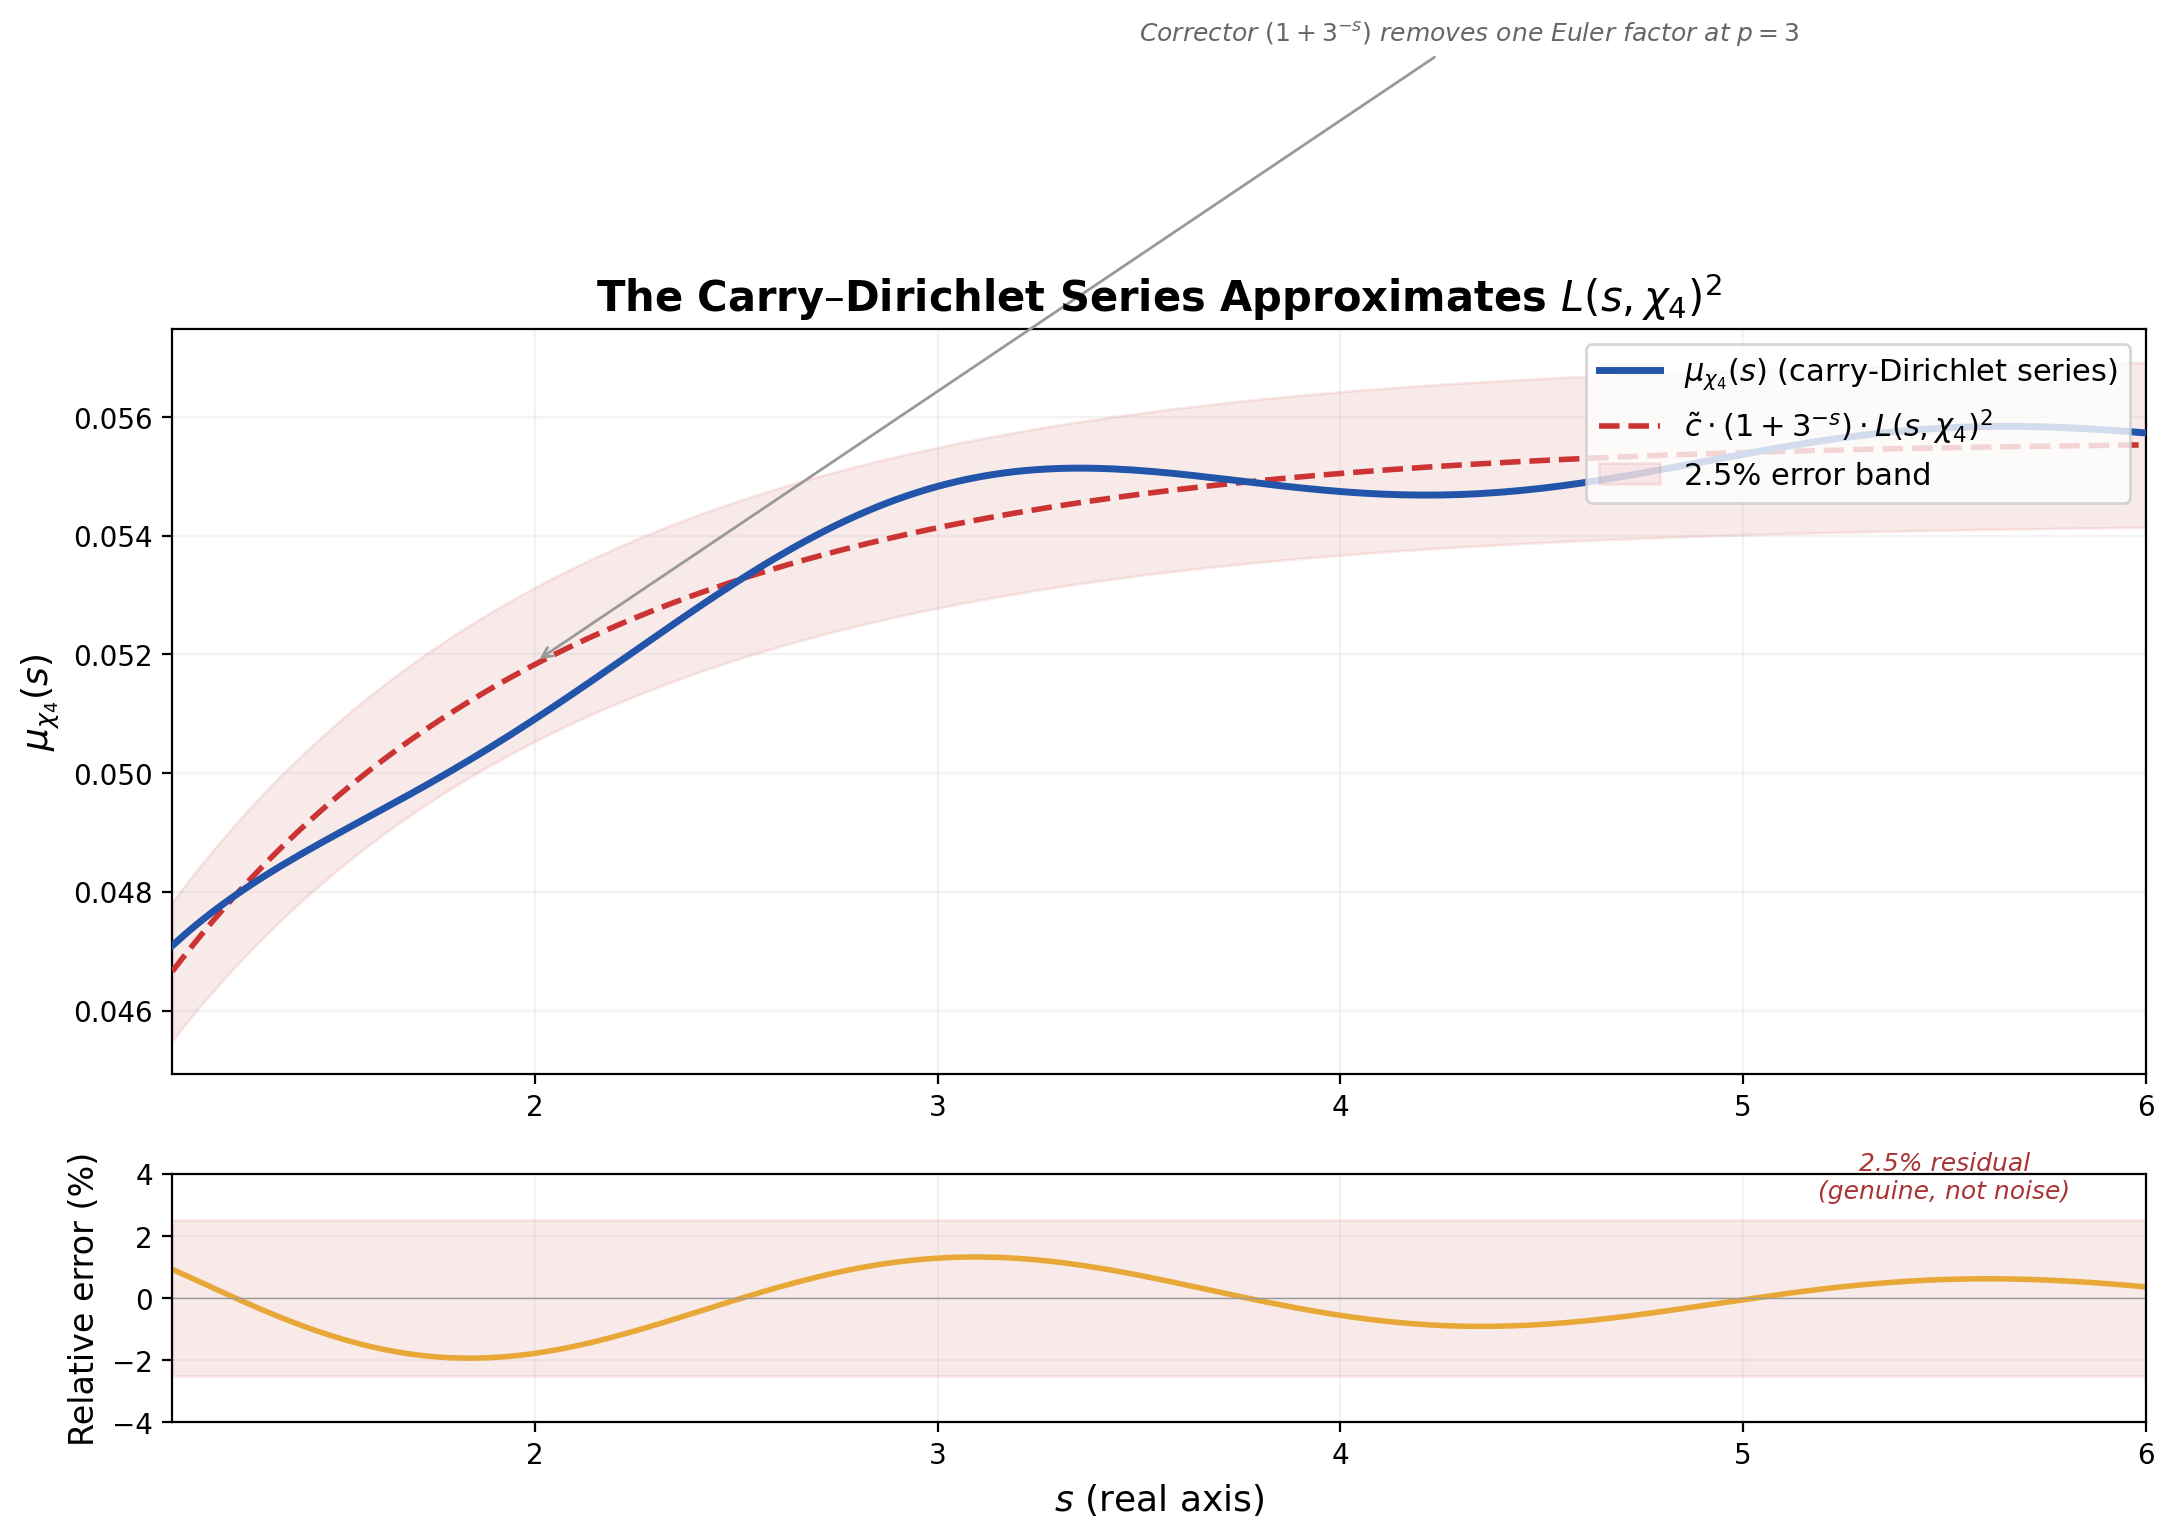
\includegraphics{../figures/fig_l_squared.png}
\caption{μ\_χ₄ vs L(s,χ₄)²}
\end{figure}

\begin{center}\rule{0.5\linewidth}{0.5pt}\end{center}

\newpage

\subsection{\texorpdfstring{5. Why \(L^2\) and Not
\(L\)?}{5. Why L\^{}2 and Not L?}}\label{why-l2-and-not-l}

The \(L^2\) structure is natural from two perspectives:

\textbf{Algebraic:} The Dirichlet series associated to a product
\(N = p \cdot q\) of two random integers is a convolution of two Dirichlet
series (one for each factor). Under the Dirichlet character \(\chi\), the
convolution becomes \(L(s, \chi) * L(s, \chi) = L(s, \chi)^2\) (up to finitely
many Euler factors).

\textbf{Analytic:} The correction factor
\(F(s) = \mu(s)/(\tilde{c} \cdot L(s, \chi_4))\) is meromorphic and zero-free in
the tested strip \([0.3, 0.7] \times [0, 15]\) (Proposition 6). Its poles
coincide with the zeros of \(L(s, \chi_4)\), confirming that the second
\(L\)-factor comes from the correction, not from the base series. The direct and
canonical carry objects themselves remain zero-free in that box.

\begin{center}\rule{0.5\linewidth}{0.5pt}\end{center}

\newpage

\subsection{6. Cross-Character Extension}\label{cross-character-extension}

The construction extends beyond \(\chi_4\):

\begin{longtable}[]{@{}llll@{}}
\toprule\noalign{}
Character \(\chi\) & Conductor & Corrector & Improvement \\
\midrule\noalign{}
\endhead
\bottomrule\noalign{}
\endlastfoot
\(\chi_4\) (mod 4) & 4 & \((1 + 3^{-s})\) & baseline \\
\(\chi_5\) (mod 5) & 5 & \((1 - \chi_5(3) \cdot 3^{-s})^2\) & +46\% \\
\(\chi_8\) (mod 8) & 8 & \((1 - \chi_8(3) \cdot 3^{-s})^2\) & +71\% \\
\(\chi_3\) (mod 3) & 3 & inert (\(\chi_3(3) = 0\)) & outlier \\
\end{longtable}

The corrector always involves \(p_0 = 3\) (the first odd prime). The conductor-3
character is an outlier because \(3 | 3\) makes the corrector trivial. The same
\((p_0,k)\) pattern is recovered from the canonical weighted-resolvent scan, so
it is not an artifact of the series presentation.

\begin{center}\rule{0.5\linewidth}{0.5pt}\end{center}

\newpage

\subsection{7. What This Does Not Claim}\label{what-this-does-not-claim}

\begin{itemize}
\tightlist
\item
  The \(L^2\) formula is a \textbf{numerical observation} with controlled error
  bounds, not a proof.
\item
  No \textbf{zero-transfer theorem} from the carry chain to \(L\)-function
  zeros.
\item
  No simple \textbf{gamma-like completion} of the canonical object produces an
  approximate functional equation on the tested mirrored grids.
\item
  No result toward the \textbf{Riemann Hypothesis} or Generalized Riemann
  Hypothesis.
\item
  The 2.5\% residual is \textbf{genuine} --- the formula is approximate, not
  exact.
\end{itemize}

\begin{center}\rule{0.5\linewidth}{0.5pt}\end{center}

\newpage

\subsection{References}\label{references}

\begin{enumerate}
\def\labelenumi{\arabic{enumi}.}
\tightlist
\item
  {[}P1{]} S. Alimonti, ``π from Pure Arithmetic: A Spectral Phase Transition in
  the Binary Carry Bridge,'' this series.
  doi:\href{https://doi.org/10.5281/zenodo.18895611}{10.5281/zenodo.18895611}
  ---
  \href{https://github.com/stefanoalimonti/carry-arithmetic-P1-pi-spectral}{GitHub}
\item
  {[}E{]} S. Alimonti, ``The Trace Anomaly of Binary Multiplication,'' this
  series.
  doi:\href{https://doi.org/10.5281/zenodo.18895604}{10.5281/zenodo.18895604}
  ---
  \href{https://github.com/stefanoalimonti/carry-arithmetic-E-trace-anomaly}{GitHub}
\item
  {[}A{]} S. Alimonti, ``Spectral Theory of Carries in Positional
  Multiplication,'' this series.
  doi:\href{https://doi.org/10.5281/zenodo.18895593}{10.5281/zenodo.18895593}
  ---
  \href{https://github.com/stefanoalimonti/carry-arithmetic-A-spectral-theory}{GitHub}
\end{enumerate}

\begin{center}\rule{0.5\linewidth}{0.5pt}\end{center}

\emph{CC BY 4.0}

\end{document}
